\newcommand{\pVSG}{\ensuremath{G_P}\xspace}
\newcommand{\lVSG}{\ensuremath{G_L}\xspace}

Unmodified, the method described above cannot handle loops for two key reasons.
%first, it brings cyclic paths, but our prior analysis only rely on acyclic path as the condition of each equality
%
First, a loop results in cyclic paths in the CFG, whereas our prior analysis relies on paths being acyclic.
%
Acyclic paths make it easy to check that the reverse program restores any desired input value no matter what path the forward program takes.
%
Secondly, our prior VSG and RG cannot represent loop control structure.
Therefore, it is simply not possible to synthesize, for example, a loop in the reverse code from the RG.
Nevertheless, we \emph{can} reuse most of the prior method by decomposing the problem suitably.
In particular, we keep the basic framework of ``SSA to VSG to RG.''
Our extension replaces SSA with a loop-enabled variant, and then extends our VSG and RG representations and algorithms to deal with cycles, thereby addressing the two aforementioned issues.
%However, there are some special steps to build the VSG for the program with loops, and the searching rule should also be updated.

Let us first assume that each loop to be reversed is a single-entry, single-exit while loop (we will explain what is a while loop later).
We explain in Section~\ref{sec:other-loops} how to convert other kinds of loops into this form.
We also assume that each loop must terminates at run-time so that we can always get an output.
Given an input while loop, there are three steps to build a VSG.
%
\begin{enumerate}

\item We temporarily collapse each while loop into a single abstract node in the CFG, thereby creating a logically loop-free CFG from which we can build a VSG by directly applying our prior method.
This ``transformation'' is for program analysis purposes only. 
We denote this loop-collapsed VSG by \pVSG.
%forming a loop-free program, and we build the VSG for it. 
%Note that this VSG only contains the input and output of each loop, but doesn't contain any value defined inside of the loop.

\item Similarly, we directly apply our prior method to build a VSG for each loop \emph{body}, which may be treated as another loop-free program.
(If the body contains nested loops, these are similarly collapsed as in Step 1 above.)
%This new VSG connects all input and output of the loop body, but doesn't contain the input and output of the loop. 
Note that path information in these loop body VSGs are local to the loop body.
We denote this VSG for the loop body by \lVSG.

\item At this point, \pVSG and \lVSG are disconnected.
Therefore, we introduce new special edges to connect them, thereby resulting in a single connected VSG.
These connecting edges are a new type of edge and constitute the main extension to our prior VSG in order to support loops.
The new edges connect each input (or output) of a loop to the input (or output) of the loop's body.
%Doing so makes it possible to retrieve the input or output of the loop through the \lVSG, thereby a loop will be generated in the reverse program.
These new edges serve as markers: when we search the VSG and produce an RG containing these edges, then we know we need to synthesize a loop.

\end{enumerate}
%
Since Steps 1 and 2 use our prior VSG construction, we need not discuss them further here.
What changes is the third step, as detailed below, including new VSG searching rules and new procedures for synthesizing loops from the search result (i.e., the RG). %We first deal with while loops then other loops.
Because state saving in a loop is very expensive, we won't consider it in a loop. Moreover, it suffices for us to deal with a single loop without nested loops, which can be handled in the same way recursively.

%Then the question is how can we connect the VSG for the whole program after reducing all loops and VSGs for loop bodies, and let the search freely traverse them to get the final VG. 


%However, in the VSG, there is no connection between the input values and output values for each loop. Therefore, our next step is building the connections between those values. We can treat each loop as another program, but we can also treat the loop body as another program. Assume this is no other loops in the loop body, so that the loop body as its own is a loop-free program which we can handle using our prior method. The third step is, how to build the special relations between the input of the loop and input of the loop body, and the output of the loop and output of the loop body. 

%To reverse a program with loops, the basic idea is similar to that for loop-free programs, but with special manipulations. From the view of the CFG, if we can reduce the loop into a single node with the same input and output, the program will turn into loop-free and will be handled in the previous way. Now what is new is how to build the VSG connecting the input and output of the loop. what we want to Specifically, the VSG built for a loop should show relationships between the input and output of the loop, and during the search if we can find a way from an input to an output or from an output to an input, we can rebuild another loop from this result producing desired values. 




%When we build a value search graph for a program without loops, each value node does contain a distinct value. However, if there is a loop, variables modified in the loop are defined more than once. Even in SSA form, a versioned variable cannot represent a single value. 

%Note that above we require that the loop has single entry and single exit, which is because such a loop has a unique input and output for each variable. 
 %In this section, we first consider a special single-entry single-exit loop: a while loop, and for other loops we will do a transformation on them on the IR level which separates the last iteration\footnote{Here we define an iteration as a control flow path from the entry of the loop header back to the same point or to the entry of an exit of the loop, and each iteration can only contain the loop header once. Hence each loop has at least one iteration at runtime.} from others. All iterations besides the last one have a single entry and a single exit, which are both the loop header, and hence can form a while loop. The last iteration will not belong to the loop and can be combined to the control flows outside of the loop.
%Consequently, we are able to handle all loops.



%Given a loop, a natural idea to get its inverse is building another loop whose body is the inverse of the body of the original loop, and those two loops should have the same number of iterations at runtime, as shown in \cite{Hou2012}, . However, there exist two problems for this approach: first, in practice, a loop may have several exits, and they may connect different control flows outside of the loop, which is difficult to reverse. %For example, consider the possibility of a reverse loop with more than one entry. 
%not have the form \texttt{while(C) S;}, where there is no side effect in \texttt{C}. Most imperative languages allow side effect existing in \texttt{C} above, and they also provide keywords allowing early exit (like \texttt{break}, \texttt{goto}, and \texttt{return} in C/C++), which results in several exits in a loop. 
%Second, if the input and output of a loop are S and T respectively, sometimes we don't want the T and S to be the input and output of the inverse of the loop, but subsets of them. To solve the first problem, we first discuss how to deal with a while loop, a special loop with single exit. For other loops we will do a transformation on them on the IR level which separates the last iteration from others, which guarantees that each iteration except the last one has single entry and single exit. To solve the second problem, we integrate the value search graph of the loop to the whole program then let the search algorithm select the input and output. 

%Our discussion of loops only considers natural loops with only one entry; loops with more than one entry are quite rare in practice and can be transformed into natural loops \cite{Muchnick}. %In this section we first deal with a standard while loop, then other loops. 


\begin{figure}%[htb]
\center{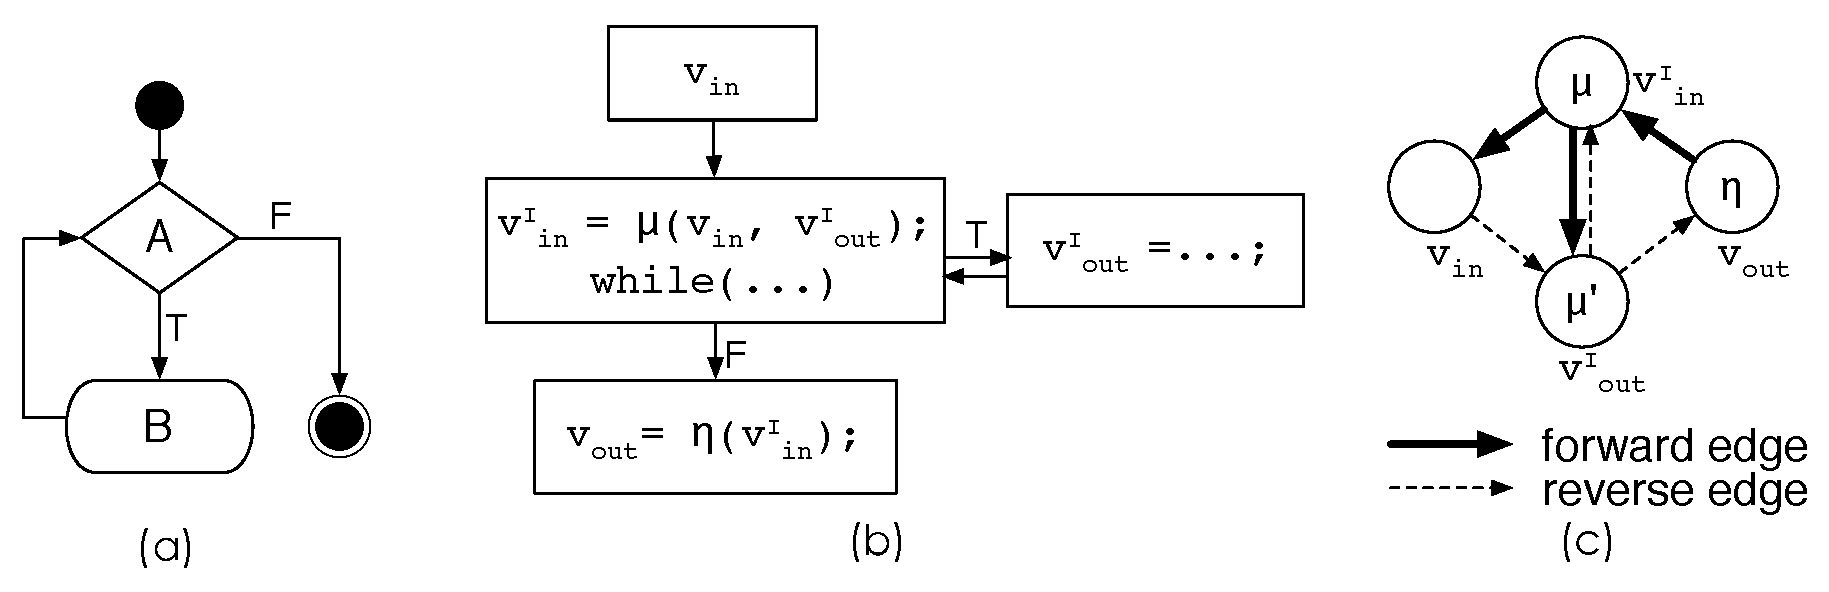
\includegraphics[width=400pt]{figures2/simpleLoop.pdf}}
\caption{(a) The diagram of a while loop. (b) The CFG in loop-closed SSA form for a variable $v$ modified in the loop. (c) Forward and reverse edges.}
\label{fig:loop_example}
\end{figure}

\subsection{Dealing with while loops}
\label{sec:while-loops}

%Let's first look at a simple while loop example. 
We first consider a while loop with the diagram shown in Figure~\ref{fig:loop_example}(a).
We further assume that $A$ has no side-effects %
%
%\footnote{A more loose condition is that a definition can exist in $A$ as long as this definition is only ``live'' in the loop, i.e., is not used outside of the loop.}
%
and that there are no escapes from $B$.
Thus, the loop only exits from its entry.  

Given such a while loop, we transform it into the \emph{loop-closed SSA form}~\cite{Pop2009}, illustrated in Figure~\ref{fig:loop_example}(b).
Loop-closed SSA differs from conventional loop-free SSA as follows.
In conventional SSA, a special marker called a \emph{$\phi$ function} is placed in the CFG at the first program point where two distinct versions (definitions) of a variable, computed along different program paths, meet.
%
In loop-closed SSA, if a value is defined inside of a loop and used outside of it, we place a special single entry $\phi$ function at the \emph{exit} of the loop.
To distinguish this type of loop-specific $\phi$ function from a conventional $\phi$ function as used in loop-free programs, we denote the loop-specific form by the term $\eta$ function, by convention~\cite{RobertA.Ballance1990}.
Additionally, suppose a definition of a variable from outside the loop and a definition coming from a back-edge of the loop meet at a program point.
Again, we create a $\phi$ function marker here, and to distinguish it, we refer to it as a $\mu$ function.

To see how these markers work, consider a variable $v$ modified by a while loop;
we now describe the corresponding loop-closed SSA form, which Figure~\ref{fig:loop_example}(b) illustrates.
Let \vinit denote the input value of $v$ before the loop executes, and \vfinal the output value of $v$ after the loop executes.
Next, let the input to the loop \emph{body} be \vmu and the output \viter.
(The superscript $I$ is intended to remind the reader that these are values associated with an \emph{iteration} of the loop, as opposed to the values before and after the loop.)
Then, \vmu is defined by a $\mu$ function as \mufunc, and \vfinal is defined by a $\eta$ function as \etafunc.
That is, \mufunc indicates the program point at which $v$ has either the initial value before the loop executes or the value produced by some iteration of the loop;
and \etafunc indicates the program point at which $v$ has the final value once the loop completes.
%We will consider the problem how to generate a forward loop 
%Now let's construct the VSG for generating the forward and reverse loops.

From this loop-closed SSA form, we wish to build a VSG that will express equality relations among the four SSA values, \vinit, \vfinal, \vmu, and \viter.
This VSG result is shown in Figure~\ref{fig:loop_example}(c).
Recall that nodes in the VSG represent values, and edges the equality relations.
%
%The loop-collapsed \pVSG comes from the left-hand column of nodes from Figure~\ref{fig:loop_example}(b) and is shown in Figure~\ref{fig:loop_example}(c) as the upper three nodes and upper two solid edges.
%The loop body \lVSG comes from the right-hand node of Figure~\ref{fig:loop_example}(b) and results in the bottom node of Figure~\ref{fig:loop_example}(c).
%
%Now we consider the problem how to retrieve \vfinal or \vinit from \lVSG.
%If we could do that, a loop will be generated in the reverse program producing \vfinal or \vinit.
%
There are four value nodes.
The nodes \vinit and \vfinal are part of the loop-collapsed \pVSG, and \vmu and \viter belong to the loop body's \lVSG.
The $\mu$ and $\eta$ functions indicate how to connect \pVSG and \lVSG.
In particular, the three solid bold edges are associated with the dependences induced by executing the loop in the forward direction;
we call these the \emph{forward edges}, and a $\mu$ node is incident to all three.
The presence of these edges make it possible to obtain \vfinal by some path passing through \lVSG, and simultaneously indicate that a loop is present for subsequent code generation.
Similarly, the three dashed edges are \emph{reverse edges} associated with dependences induced in the reverse direction.
These edges make it possible to obtain \vinit by some path through \lVSG.
Note that the reverse edges form a symmetry to the forward edges.
From this symmetry, we define the node incident to all three reverse edges as a $\mu'$ node.
Later we will show how the search traverses these edges.

Having built the CFG, the next step is to search it, producing the RG result.
Recall that we are given a set of target nodes whose values we wish to eventually compute from a starting set of available nodes.
We search for a path from available nodes to target nodes; the subgraph representing paths is the RG, which is not necessarily unique.
Our algorithm is similar to the one we have described previously~\cite{Hou2012}, but for loops we need three additional search rules:

\begin{itemize}
\item During a search for a value, once a forward/reverse edge is selected, all edges in the other category cannot be chosen. This is because either a forward or a reverse loop will be built to retrieve the value.

%To build a forward loop, if the search reaches a $\mu$ node, it forks by advancing through the two outgoing forward edges; to build a reverse loop, if the search reaches a $\mu'$ node, it forks by advancing through the two outgoing reverse edges. 
\item When the search reaches a $\mu$ or $\mu'$ node, it will be split into two sub-searches, in \pVSG and \lVSG, respectively, through the two outgoing forward or reverse edges.
For example, in Figure~\ref{fig:loop_example}(c), if the search reaches \vmu, the algorithm begins two sub-searches beginning with \vinit and \viter.

%As we discussed above, if at compile time we can determine that the loop body will certainly be traversed at runtime, the search does not fork but continues toward \viter or \vmu.
\item During the search, the algorithm may form a directed cycle only in \lVSG; furthermore, such a cycle must contain a forward or reverse edge between a $\mu$ and $\mu'$ node. 
Once a cycle is formed, the search in \lVSG is complete.
%will not move further from the current node just like when an available node is reached.
\end{itemize}

\noindent
We build a while loop as either a forward or a reverse loop. 
Synthesizing such a while loop consists of synthesizing its body and predicate.


\subsubsection{Building the loop body.}

The loop body in the reverse program is generated from the search result in \lVSG.
For each variable we remove the edge between the $\mu$ and $\mu'$ nodes and hence remove the cycles, so that we can generate the loop body using our prior code generation algorithm.

%there is no cycles any more. 
%As a result, this subgraph of the RG used to build the loop body connects each \viter or \vmu (for forward or reverse loop) to the $\mu$/$\mu'$ node or value nodes not defined in the loop. The code is generated in the same method as in \cite{Hou2012}. 
%Since recording control flows in a loop may be expensive, we will use the method mentioned in the previous section which retrieves each value in the predicate. If this method does not work, we have to record the control flows for all iterations using a bit vector. It is possible that the cost to store control flows offsets the benefit to retrieve a value from a loop which may not need a state saving. In this case, we can turn to the method in \cite{Hou2012} which is a better choice.

\begin{comment}

\begin{figure}%[htb]
\center{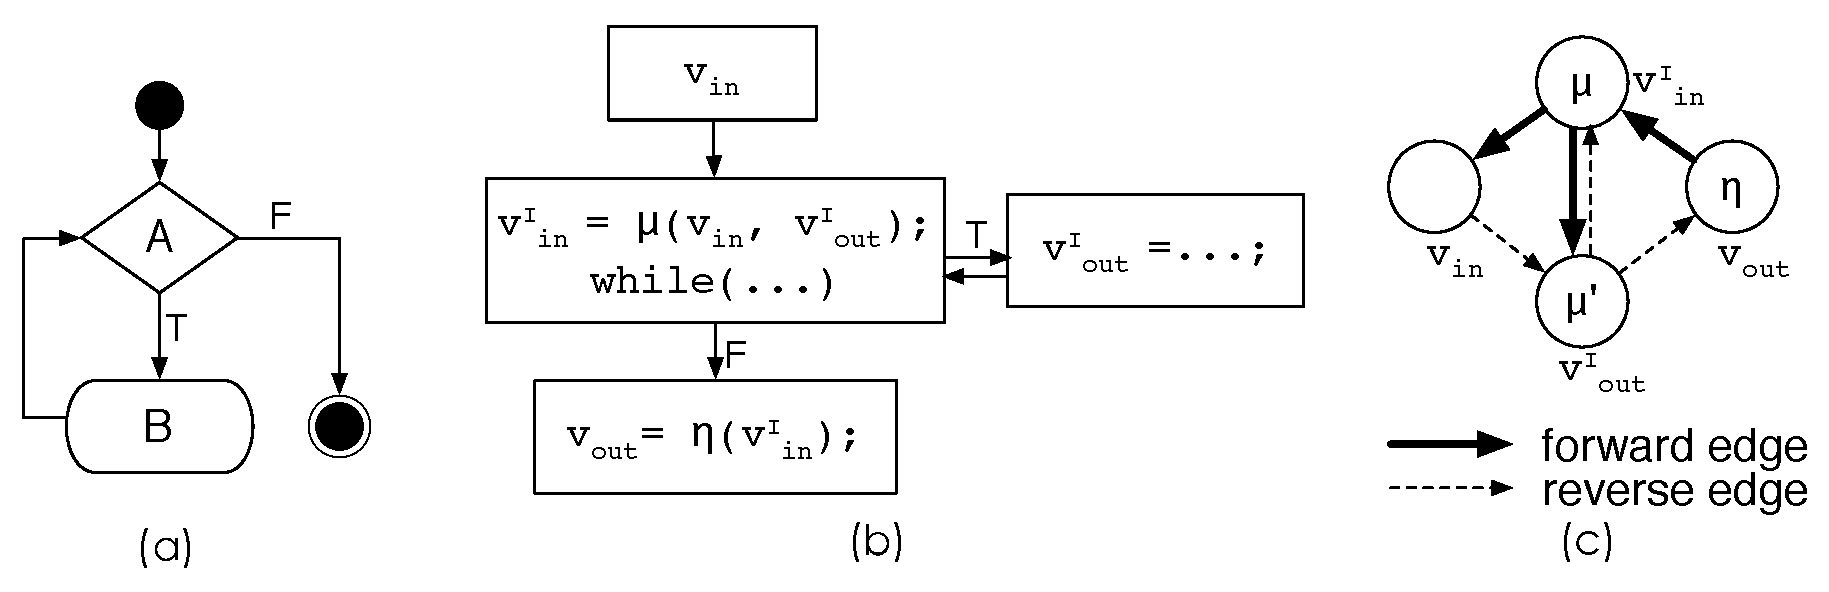
\includegraphics[width=300pt]{figures2/loopExample.pdf}}
\caption{(a) The VSG for our example. (b) The RG for retrieving $a_3$ and $i_3$. (c) The RG for retrieving $a_0$.}
\label{fig:loopExample}
\end{figure}

\end{comment}



%Our search begins from the node $a_0$ in Figure \ref{fig:loop_vsg}(a). Once we go from $a_0$ to $a_1$ into the loop block\footnote{\TODO{need we define this term?}}, we are selecting to build a reverse loop, and we will add some restrictions during the search: all edges belonging to the forward execution should not be taken. 

%In [], we forbid any circle during the search for each CFG path, however, since we are building another loop, we permit the circle to appear in the search result, with one requirement: each circle should contain the edge between $v_{\mu}$ and $v_{iter}$.



%The loop body generated from Figure \ref{fig:loop_vsg}(b) is \texttt{\{ i = i + 1; a = a + i;  \}}, and the loop body generated from Figure \ref{fig:loop_vsg}(c) is \texttt{\{ a = a - i;  i = i - 1; \}}.


\subsubsection{Building the loop predicate.}

To guarantee that the generated loop has the same iterations at runtime as the original loop, we need to build a proper loop predicate. 
We propose three approaches to building a correct loop predicate. 
To illustrate those approaches, we temporarily introduce the following loop example. We assume that the omitted statements  modify neither \texttt{A[]} nor \texttt{i}.

\begin{lstlisting}
i = 0;
while (A[i] > 0) {
    /* ... */
    i = i + 2;
}
\end{lstlisting}



%The first two approaches are preferred since they may not need any instrumentation to the original loop, but cannot be always applied, and the third one needs an instrumentation to the forward program and is always working. 

\begin{itemize}
\setlength{\itemsep}{5pt}%

\item \textbf{Approach 1:} Building the same loop predicate as that in the original loop. 
To build this predicate, we need to retrieve each value in the predicate.
%, we need to retrieve its input value of the loop before the loop, and if it is updated in the loop, we also need to retrieve its input value of the loop body in the loop. 
A new search is needed to acquire those values, and the search result will be combined into the RG generated above.
For the example above, we can build a loop below that has the same number of iterations as the original one. The omitted statements will be substituted by the loop body built above.


\begin{lstlisting}
i = 0;
while (A[i] > 0) {
    /* ... */
    i = i + 2;
}
\end{lstlisting}



%In the second case, we  
%$a$ for example, if it is not modified in the loop, we need to retrieve the value of $a$ before building the while condition; if it is defined by a $\mu$ function as $a_{in}^I = \mu (a_{in}, a_{out}^I)$, both $a_{in}$ and $a_{out}^I$ should be retrieved. 
%Figure \ref{fig:rvsLoops}(a) shows the resulted loop built from this approach.
%This is done by starting another search beginning with $a_{in}^I $. Note that we also updated the loop body to include the statement that defines $a_{out}^I$.


\item \textbf{Approach 2:} Building the loop predicate from a variable updated in the loop. Given a variable $v$ and its four definitions: \vinit, \vmu, \viter, and \vfinal, if \vmu$\ne$\vfinal in each iteration except the last definition of \vmu (which is actually \vfinal), and if we can retrieve \vinit and \vfinal before the loop (hence we cannot retrieve them through the loop), and \viter in the loop, we can use them to build a while loop as:
$$
u := v_{in}; \;\\
while (u \ne v_{out}) \;  \{\; 
/* \; update \; u \; */ \; 
\}
$$

Similarly, if \viter$\ne$\vinit  in each iteration, and  \vinit and \vfinal can be retrieved before the loop, and \vmu can be retrieved in the loop, we can use them to build a while loop as: 
$$
u := v_{out}; \; while (u \ne v_{in}) \;  \{\; /* \; update \; u \; */ \; \}
$$

In general, it is difficult to detect all variables satisfying the properties above.
However, there are some special cases.
One case is that of \emph{monotonic variables}~\cite{Wolfe1992}, which are monotonically strictly increasing or decreasing in each iteration.
Another is that of induction variables, which are special monotonic variables that are relatively easier to recognize. In the above example, \texttt{i} is an induction variable. Assume its final value after the loop is \texttt{i1} that is known, and then we can build the following loop with the predicate using \texttt{i}.



\begin{lstlisting}
i = 0;
while (i != i1) {
    /* ... */
    i = i + 2;
}
\end{lstlisting}


%Indeed, the first approach above is a special case of this one if we define another Boolean variable $c$ as $a < b$, where $c$ satisfies the condition above.
 %Instead, we only detect variables which are updated during iterations monotonically. Note that induction variables fall into this category which are easier to detect.
%loop variant. A loop variant is a variable whose value is updated in each iteration monotonically\footnote{This is too strict: \TODO{distinct values are also OK.}} and the while condition is a comparison between the loop variant and another value. Assume the loop variant is $i$ with initial value $i_{init}$ and final value $i_{final}$, and in all iterations, $i$ is increased or decreased monotonically. If we can retrieve $i_{init}$ and $i_{final}$, plus $i_{\mu}$ or $i_{iter}$ in each iteration, we can use this variable to build the while condition for the forward or reverse loop. Specifically, a forward loop \TODO{Note that it does not make sense to classify a loop as a forward or reverse one, since they may appear in the same loop} is built like:
%To build the while condition, we first detect all loop variants in the loop (\TODO{how?}). For each loop variant $i$, we have to retrieve both $i_{init}$ and $i_{final}$, and depending on whether the generated loop is forward or reverse, we have also to retrieve either $i_{\mu}$ or $i_{iter}$. 
%Because at the beginning of the loop, we should already have $i_{init}$ and $i_{final}$, we cannot retrieve them through the loop. This means the search should not reach the loop nodes from them. The search for $i_{\mu}$ or $i_{iter}$ follows two forward or reverse edges as described above. 
%In case that there are several candidates satisfying the requirement above, for each variable, we calculate the cost to retrieve all dependent values and choose one with the least cost to build the loop predicate. 
%In our example, both $a$ and $i$ are monotonic variables, but  $a$'s initial value is unknown (which is what we are retrieving!). In contrast, $i$'s initial and final value are 0 and $N$, and $i$ can be updated either by a forward loop beginning with its initial value, or a reverse loop beginning with its final value. Figure \ref{fig:rvsLoops}(b) and (c) shows those two results. Note that in Figure \ref{fig:rvsLoops}(c) the code retrieving $i$ in the loop body is shared with the loop body generated before \TODO{!}.


\begin{comment}
\begin{figure}%[htb]
\center{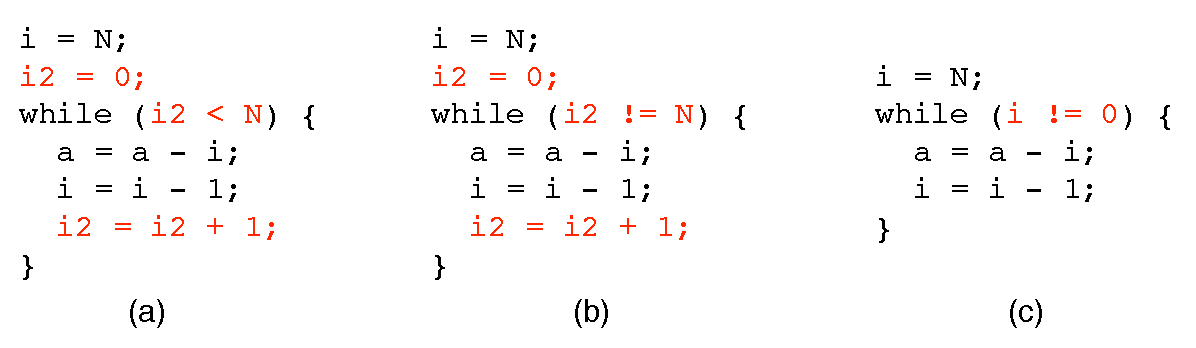
\includegraphics[width=300pt]{figures2/reverseLoops.pdf}}
\caption{Three results.}
\label{fig:rvsLoops}
\end{figure}
\end{comment}

%However, it is possible that we cannot find such a loop variant. (Although every loop that terminates has a variant). 
%The reason is that the loop variant we are looking for is somehow special, but it is possible \TODO{see wiki: Transfinite induction}. 
\item \textbf{Approach 3:} Instrumenting the original loop with a counter counting the number of iterations. The counter has the initial value zero and is incremented by one on each back edge of the loop.
The final value of the counter is stored in the forward program and restored in the reverse program as the maximum value of another loop counter.
This approach generally works if either of the above two approaches fail.
However, it requires instrumentation (the counter), and therefore forces generation of a forward program. Below we show the instrumented loop in the forward program (first) and the generated loop in the reverse program (second) for the above example.

\begin{lstlisting}
i = 0;
count = 0;
while (A[i] > 0) {
    /* ... */
    i = i + 2;
    count = count + 1;
}
\end{lstlisting}


\begin{lstlisting}
while (count > 0) {
    /* ... */
    count = count - 1;
}
\end{lstlisting}


\end{itemize}

We prioritize these approaches as follows.
Applicability and state-saving cost are our main criteria.
We prefer Approach 1 and 2 over 3.
When either 1 or 2 apply, if no state-saving is required, we apply them.
Otherwise, we try Approach 3 and choose the overall approach with the least cost.

\vspace{3mm}

\begin{figure}%[htb]
\center{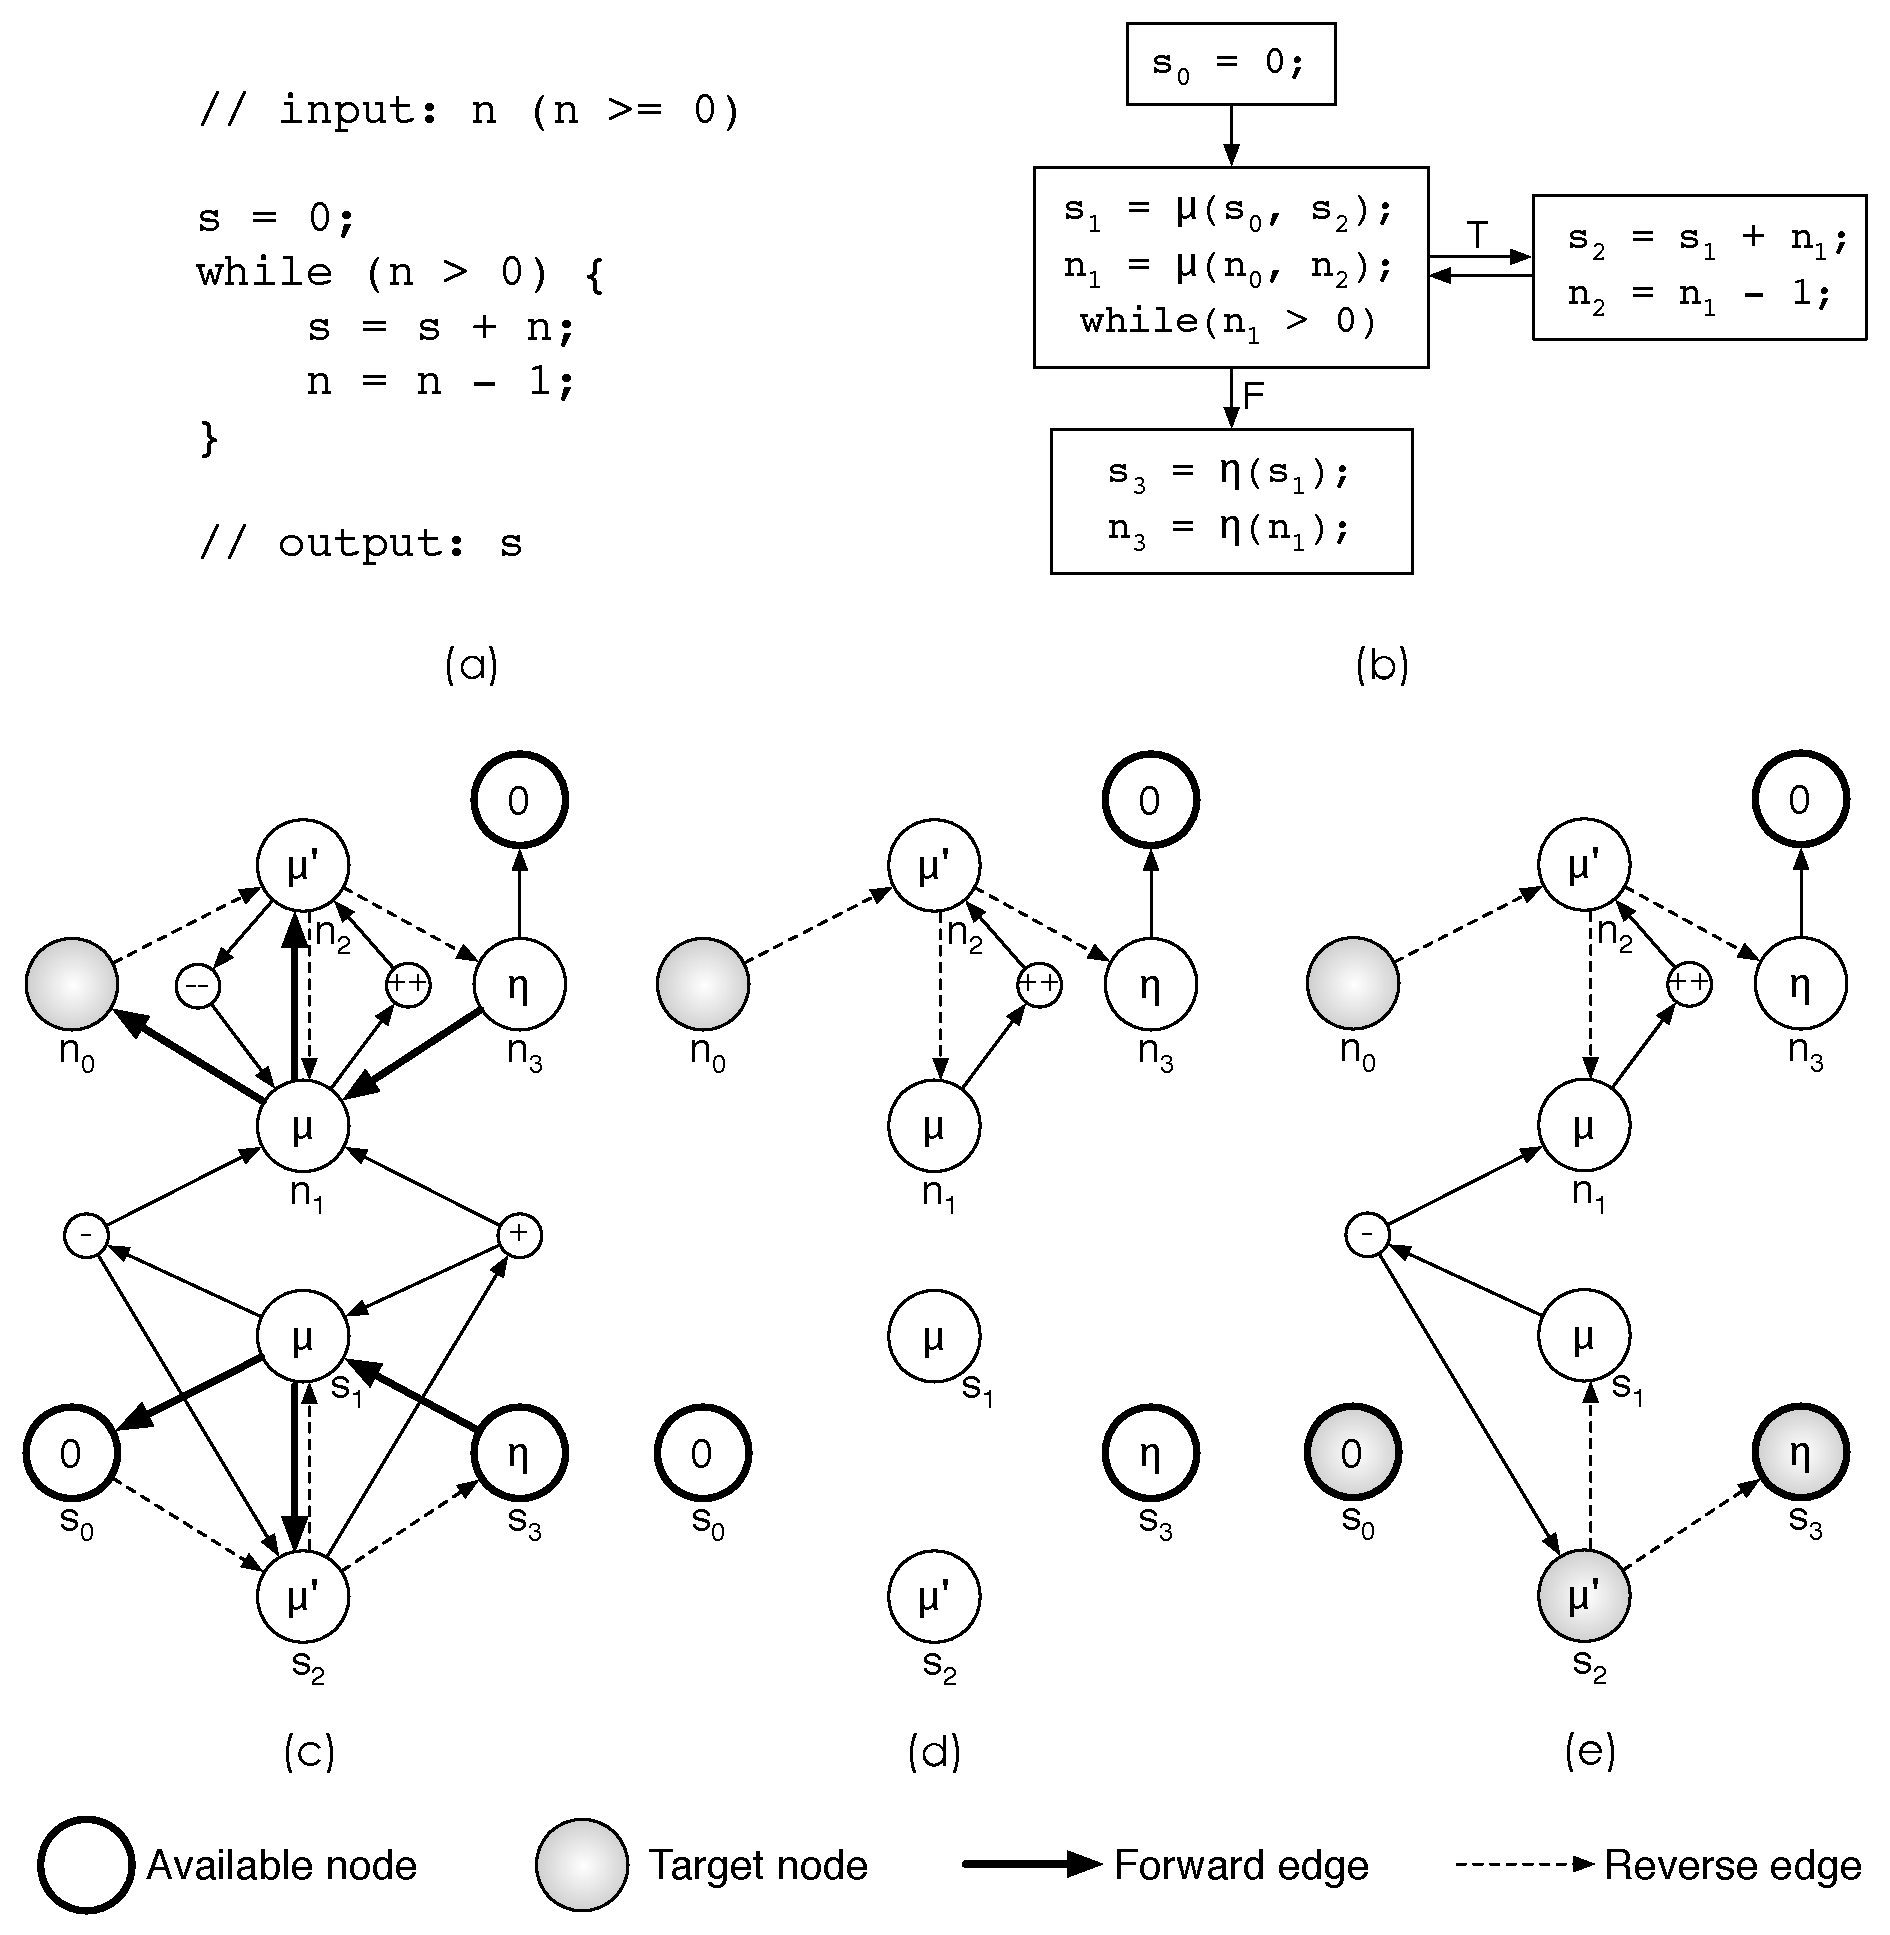
\includegraphics[width=400pt]{figures2/loopVSG.pdf}}
\caption{(a) The program of our example. (b) The CFG in loop-closed SSA form. (c) The VSG.  (d) The RG for retrieving $n_3$. (e) The RG for retrieving $n_0$ and $s_2$.}
\label{fig:loop_vsg}
\end{figure}

As an example, suppose we apply this algorithm to the loop in Figure~\ref{fig:loop_vsg}(a).
Figure \ref{fig:loop_vsg}(b) shows its CFG in loop-closed SSA.
The input is $n_0$ and the output $s_3$.
Our goal is to generate a reverse program that takes $s_3$ as input and produces $n_0$.
We build the VSG shown in Figure~\ref{fig:loop_vsg}(c), with forward and reverse edges shown as bold and dashed edges, respectively.
Note that the equality between $n_3$ and 0 is acquired from solving constraints, a standard compiler technique.%
%
\footnote{For clarify, we remove the equality $n_1=s_2-s_1$, as this relation will not be used during the search.}
%
The search result for value $n_0$ is shown in Figure \ref{fig:loop_vsg}(d), from which we can build the loop body as \texttt{\{ n = n + 1;  \}}.

Next, we build the loop predicate.
In our example, because we wish to retrieve the initial value of $n$, we cannot use it to build the loop predicate.
We can discover that $s$ is a monotonic variable, and that both the initial and final values of $s$, which are 0 and $s_3$, respectively, are available.
To get $s_2$, we search its value on the VSG and the search result is shown in Figure \ref{fig:loop_vsg}(e). 
As a result, we build the loop predicate from $s$ and the reverse program is generated as below.


\begin{lstlisting}
while (s != 0) {
    n = n + 1;
    s = s - n;
}
\end{lstlisting}


Above we have built a reverse loop in the reverse program, but it is also possible that the reverse program contains a forward loop. 
For instance, if we change our example into the program shown  below:


\begin{lstlisting}
s = 0;
i = 0;
while (i < n) {
    i = i + 1;
    s = s + i;
}
\end{lstlisting}


Without modifying its semantic, its inverse will contain a forward loop which is shown below:

\begin{lstlisting}
s2 = 0;
i = 0;
while (s2 != s) {
    i = i + 1;
    s2 = s2 + i;
}
n = i;
\end{lstlisting}

 This is because the input of the new program $n_0$ is equal to $i$'s final value, which is the output of the loop. 

%\subsubsection{Other single-exit loops}
%The while loop we discussed above is just one kind of the single-exit loops. %Do-while loop is another single-exit loop. 
%For other single-exit loops, we can transform them into while loops, and we can also utilize the similar technique as above to handle them. However, as we will see later, the transformation described below can handle those cases including loops with several exits. 

\subsection{Dealing with loops other than while loops}
\label{sec:other-loops}

In practice, the vast majority of loops have a single entry, which are called \emph{natural loops}~\cite{Muchnick}. 
Loops with more than one entry are quite rare and can in fact be transformed into natural loops~\cite{Muchnick}. 
However, it is quite common that a loop has several exits. 
For example, in C/C++ we may exit a loop early through \texttt{break}, \texttt{return}, or \texttt{goto} statements.
Nevertheless, given a non-while natural loop, we can transform it to separate the last iteration from the loop;
then, the remaining iterations form a new while loop, and the last iteration will not belong to the loop and hence can considered with the control flows outside of the loop. 
We then process the new while loop as previously described.
Note that this ``transformation'' is only applied to the CFG during the analysis, and not to the original program.
As such, in the forward program \Forward the last iteration and other iterations of each loop continue to share the same code.


Figure~\ref{fig:loop}(a) shows a loop in a CFG, with a header (node 1) and two back edges (4$\to$1 and 5$\to$1). 
There are two different exits from this loop, which are nodes 6 and 7.
%An exit edge of a loop is an edge connecting a loop node to an exit. 
%1$\to$6 and 3$\to$7 are two exit edges.
Figure~\ref{fig:loop}(b) shows the CFG of the transformed loop.
This transformation is performed as follows.

In a natural loop, only the last iteration takes the exit, and any other iteration goes back to the loop header.
Therefore, if the last iteration is peeled off from the loop, this loop will turn into a while loop. 
%Suppose we can predicate the number of iterations (the number of back edges being traversed) before a loop is taken, which is although impossible for most loops. Let \texttt{k}  be a virtual variable whose value is the number of the back edges being taken at runtime, 
To implement this transformation, we create a new branch node with an unknown predicate that returns $true$ if the next iteration is not the last one and $false$ otherwise.
Note that we will not build this predicate in the forward program. 
The new branch node turns over all in-edges of the loop header. 
%Note that  \texttt{k}'s initial value usually cannot be determined at compile time, but we are not actually doing this transformation to the original function and hence it won't bring any problem here. 
Its $true$ labeled out-edge will point to the loop header of a copy of the loop (node $1'$) with back edges but without exit edges, and all back edges are redirected to this new branch node making it a new loop header. 
Note that after removing exit edges it is possible that a previous branch node becomes a non-branch node (node $3'$, for example), which is fine because the removed branch edge will not be taken. Then, we can remove the (side effect free) predicates from those nodes. The edge labeled with $false$ from the new branch node will point to the original loop header (node 1) and all back edges in the original loop are removed, since the last iteration won't take the back edge. The nodes from which the exit of the program is not reachable due to the back edge removal are removed (node 4 and 5, for example). Again the predicate is removed from a node once it is not a branch node anymore (node 2 and 3).
%Fig \ref{fig:loop}(b) shows the transformed flow graph where the node 0 is the new branch node and loop header. Note that the node 4 and 5 are removed since they are not reachable anymore.
 %At runtime, the true edge must be traversed and the false edge may not. 
%The true edge postdominates the false edge, but the latter does not dominate the former. 

\begin{figure}%[htb]
\center{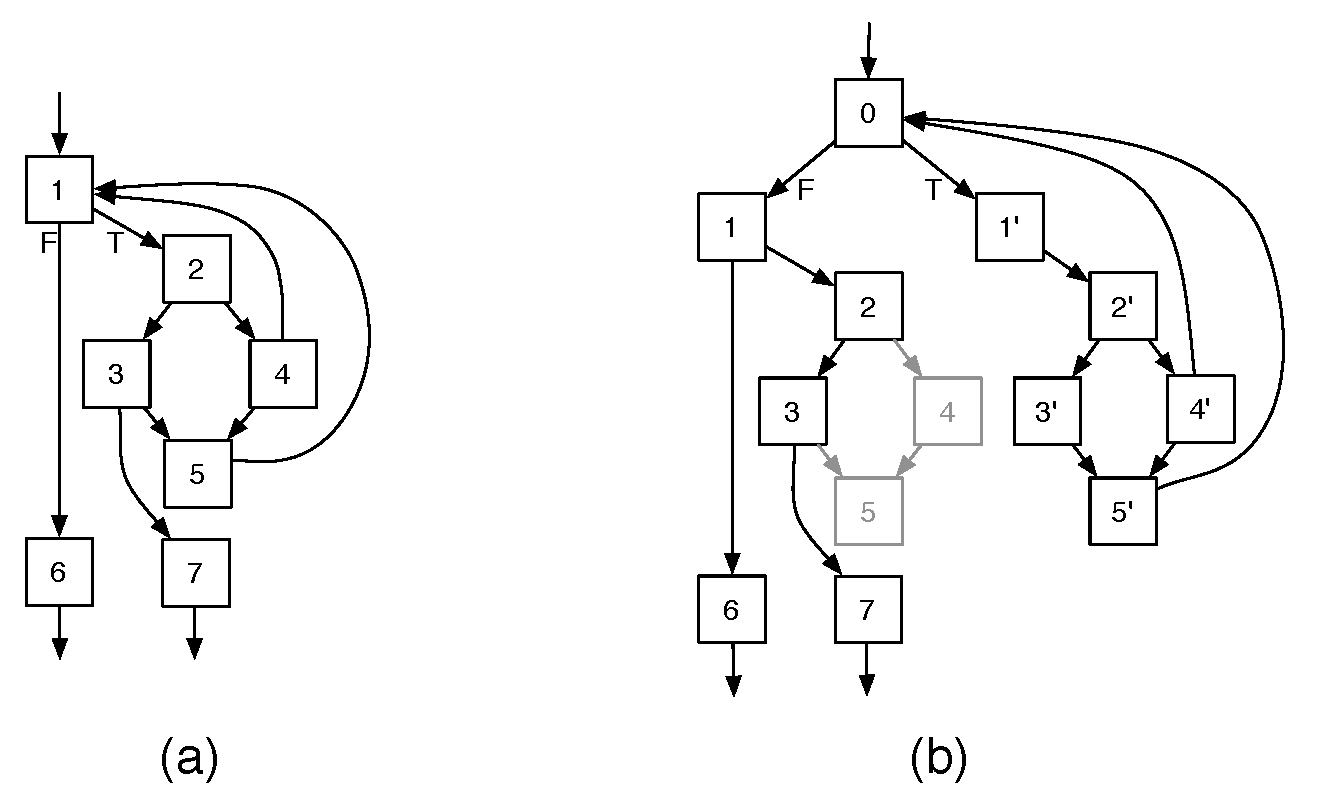
\includegraphics[width=350pt]{figures2/Loop.pdf}}
\caption{(a) A loop in CFG with two back edges and two exits. (b) The CFG of the transformed loop.}
\label{fig:loop}
\end{figure}

After the transformation, all loops in the program become while loops and our method applies.
Since the new generated loop predicate  is unknown, to build the loop predicate  in the reverse program, we cannot use the first approach proposed above any more. %Therefore, it is preferred that a loop be transformed into a while loop normally, not in the above method. For example, a do-while loop can be easily converted into a while loop.

Because those two newly created branch bodies share the same code in the forward program,  any instrumentation will also be shared between them. 
For example, if a value defined in the false body above needs a state saving, in the forward program we can only perform the state saving in the loop, which results in saving a value many times and then larger time overhead. 
For this reason, we could forbid state savings on any variable in the false body.
Properly defining the cost of this operation may help to get the better search result. 
%On the other hand, if a state saving is made from reversing the loop hammock, at the exit of the loop, any side effect should be taken care. For example, if a stack is used to store variables, the pop operations may be needed at the exits.

